\begin{center}
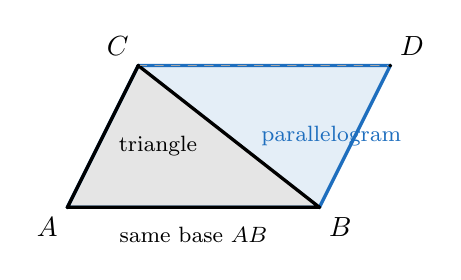
\begin{tikzpicture}[scale=1.0, line cap=round, line join=round]
  \definecolor{euclidblue}{RGB}{30,110,190}
  \coordinate (A) at (0,0);
  \coordinate (B) at (3.2,0);
  \coordinate (C) at (0.9,1.8);
  \coordinate (D) at (4.1,1.8);
  \fill[euclidblue!12] (A)--(B)--(D)--(C)--cycle;
  \fill[gray!20] (A)--(B)--(C)--cycle;
  \draw[very thick, euclidblue] (A)--(B)--(D)--(C)--cycle;
  \draw[very thick] (A)--(B)--(C)--cycle;
  \draw[gray!70, dashed] (C)--(D);
  \foreach \p/\pos in {A/below left,B/below right,C/above left,D/above right}{
    \fill (\p) circle (0.025);
    \node[\pos] at (\p) {$\p$};
  }
  \node[font=\footnotesize] at (1.6,-0.35) {same base $AB$};
  \node[euclidblue, font=\footnotesize] at (3.35,0.9) {parallelogram};
  \node[font=\footnotesize] at (1.15,0.78) {triangle};
\end{tikzpicture}
\end{center}
